%%
%% Copyright Guy Taylor 2012
%%
%%

\chapter{Design}

\section{The Goal}
My task was to design and implement a low power wireless network for the Respire devices. This
network should be effective in both reducing the power consumption of the Respire device and
allow the required data to be accessible in real-time. An extension of the design should allow bulk
data upload if the device re-enters the network after a period of disconnection. The network should
also allow a simple device initialisation within the network, so as to be as ``plug-and-play'' as possible
and also allow the device to actively maintain a connection as the patient moves between relays or
networks. The network should allow relay devices to extend the signal from the data collection
destination, so simplifying any wiring requirements.

\section{Requirements}
The Respire is intended to be used initially in a hospital environment but with the hope to later
extend it for use in a patient's residence. There is therefore a requirement for it to be legal for public
use with no assumption of consistent infrastructure. Within hospitals it is required not to interact
with other equipment or prevent use of required services.


The Respire should be as simple as possible as the user at home is not expected to be
knowledgeable in the area and the medical professional should not be burdened with configuration
or maintenance. This also reduces both cost and chance of failure, enabling access to more patients
and reducing patients risk during failures.


The Respire network should allow the patient greater freedom to move around a room or building
without the need to be tethered to sensor, power or communications equipment. This should help
promote mobility and, in consequence, aid recovery and reduce hospital stay.
The Respire should be able to produce real-time data when needed but also be able to store and
then later transmit the data when connections permit. A fully functioning Respire network needs to
be capable of transmitting 3x14-bit samples at sample rate of 12.5Hz for effective respiratory
monitoring (Mann, J; personal communication).


\section{The Device}
The Respire consists of a single self contained \ac{PCB} with attached battery. The PCB contains the
central microcontroller, low power radio with antenna, three-axis accelerometer and flash storage.
At every level the Respire tries to reduce the power needs (\eg by reducing the chip count), and thus
each device selected is designed to be used in low power environments. Attributes of the Respire
include:\\
\textbf{Strengths}
\begin{itemize}
  \item A single 32-bit ARM Cortex-M3 microcontroller, enabling local data processing.
  \item All low power chips by design.
  \item Devices have low power sleep states, including four in the microcontroller.
  \item The radio transmits with a high bandwidth, allowing shortened duty cycles.
\end{itemize}
\textbf{Weaknesses}
\begin{itemize}
  \item Proprietary radio \ac{PHY}/\ac{DL} layer, non-standard and sufficiently different to prevent implementation of a standard.
  \item Problematic state machines due to sleep states.
\end{itemize}

\section{Network Design}
\begin{wrapfigure}{r}{0.7\textwidth}
  \vspace{-10pt}
  \begin{center}
    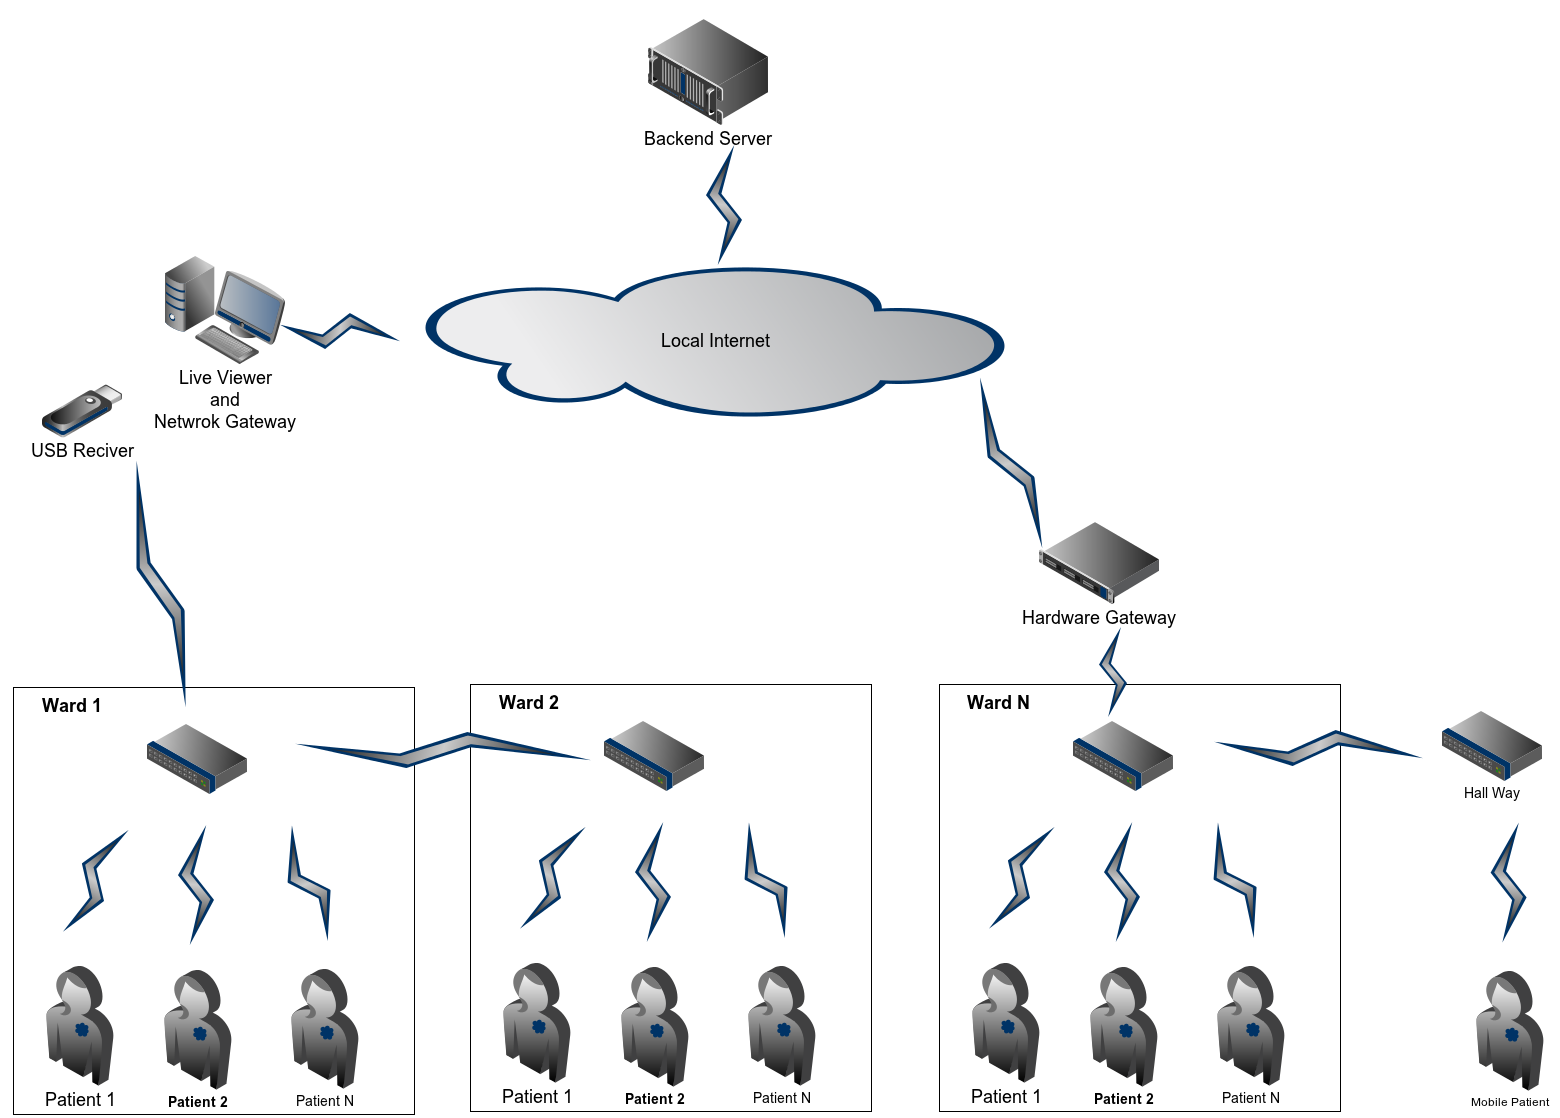
\includegraphics[width=0.6\textwidth, keepaspectratio=true]{images/respire_network.png}
  \end{center}
  \caption[Network Design]{Network design}
  \vspace{-10pt}
\end{wrapfigure}
In this project I will propose a design for a low power wireless network system, this will be laid out in
a layered approach. Due to the unique hardware of the Respire no previous network has been
produced at the time of commencing this project address an entire radio stack by designing the
separate layers up the design will try and separate out the separate components creating a layered
and modular approach.

\subsection{Multiplexing}
As many Respire devices will be working in the same area there is a requirement that some sort of
multiple access system is implemented. In the wireless, and wired, domain there are three main
groups of multiplexing; \ac{TDMA}, \ac{FDMA} and \ac{CSMA}.

\subsubsection{\acf{FDMA}}
FDMA separates the signal spectrum into several channels, each with its own unique frequency
range. Each separate device then only transmits in its allotted channel. This provides the maximum
single throughput per device but comes with the requirement of either a separate receiver per
frequency or a more-expensive and energy-intensive broad frequency receiver. \ac{FDMA} is typically
used in managed environments, where one can guarantee each device has its own frequency.
\ac{FDMA} cannot be effectively implemented on the \ac{NRF24} as it cannot receive on more than one
channel and channel-hopping would be less effective than \ac{TDMA}. This would however reduce the
risk of noise on a single channel that \ac{TDMA} is susceptible to.

\subsubsection{\acf{CSMA}}
\ac{CSMA} has several variations all based around a single concept; that is, a device that wishes to
transmit, first senses the spectrum to ascertain whether it is free to transmit and if so, transmits its
data. The different variations diverge in respect to how they handle the situation if another device is
transmitting or the situation where more than one device has transmitted at the same time.
A key issue with \ac{CSMA} is the ``hidden terminal problem'', where two devices out of range of each
other but visible to a third compete for spectrum. One of the possible mitigation schemes is to use a
mediation device to share node information more globally in the network without high memory
costs, this could be achieved.


\ac{CSMA} however is not possible on the \ac{NRF24} as it does not adequately provide this built-in
ability or an effective equivalent software alternative to sense the channel. This would reduce the
need for accurate clocks and a highly managed \ac{TDMA} solution.


\subsubsection{\acf{TDMA}}
\ac{TDMA} allocates a time slot for each device, or as requested, for a single device to transmit within
uniquely. This distribution allows many devices to use a single channel without the need for sensing
or frequency change. However it requires an accurate time to be kept, and implemented on, for the
bandwidth to be used effectively. The requirement for accurate timekeeping and synchronisation
causes the greatest challenge for this type of multiplexing, because in modern electronics each
crystal (the component used to track time) has its own unique characteristics. The inability to keep
the clocks synchronised without adjustment can cause one device to transmit in another's time slot.
Time division multiplexing in its simplest form is most efficient when the data being transmitted is
both consistent and equally shared among the timeslots. This can be mitigated by giving devices that
need more bandwidth longer time periods but this requires predictable data requirements.
\ac{TDMA} also has an intrinsic but fixed maximum latency in communication and so can be used in time
critical applications, such as telecommunications. This benefit however, can only be achieved if each
device can be serviced in sufficient time before the cycle repeats. This often leads to \ac{TDMA} being
used in high frequency spectrum.


\ac{TDMA} was chosen for the Respire network as the radio can transmit at precise intervals and the
microcontroller provides an accurate clock. This choice had the benefit of allowing the network to
choose the least congested frequency band within the overcrowded \ac{ISM} bands and effectively
utilises Respires low power devices.

%TODO 
%{discussion of why TDMA}


\subsection{\acf{PHY} layer}

\begin{wrapfigure}{r}{0.5\textwidth}
  \vspace{-10pt}
  \begin{center}
    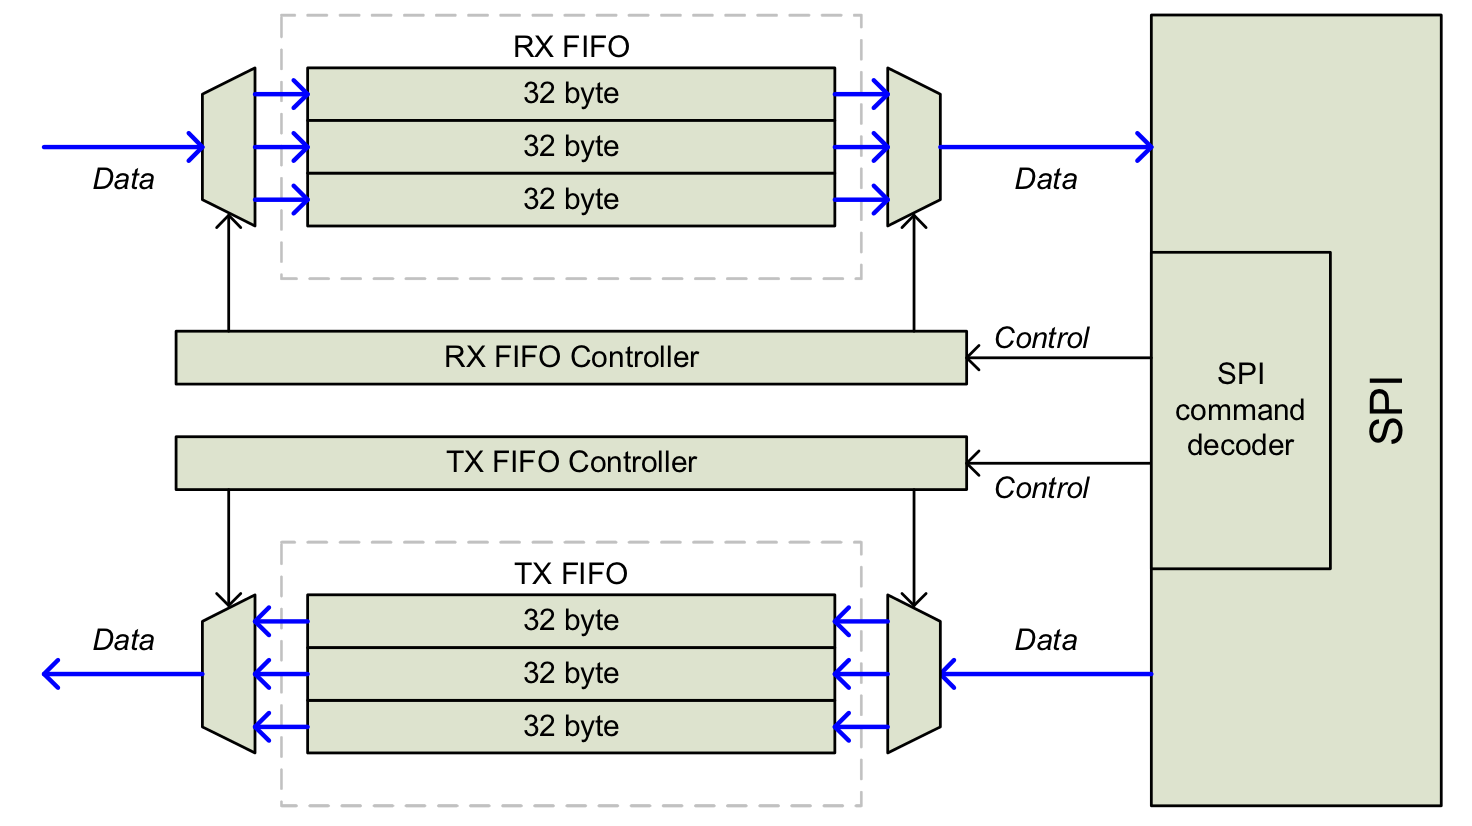
\includegraphics[width=0.4\textwidth, keepaspectratio=true]{images/nrf24_pipline.png}
  \end{center}
  \caption[\ac{NRF24} Pipline]{\ac{NRF24} pipline\citer{NRF24Spec}}
  \vspace{-10pt}
\end{wrapfigure}

The \ac{PHY} layer of the \ac{NRF24} has many unique hardware features and to reduce power
it was decided to attempt to integrate these as much as possible.


The chip supports up to six separate receive pipelines each with its own address. This is designed to
support a small, many transmitters to single receiver, network (\eg Logitech's Unifying\textsuperscript{\textregistered} brand of
wireless keyboards and mice). There are six separate receiving addresses but only two of these can 
be independently configured. This solution was therefore not used as the restriction of a network
size to six nodes per repeater was inadequate.

An unusual feature of the chip is the use of the address as the sync in the air. This increases the
packet efficiency as it removes sections unused by the \ac{DL} layer and instead uses them instead. This
however restricts the address choices at the DL layer and disables any packet sniffing for debugging
or more custom \ac{DL} layer. As the address is sued as the sink pattern there is a need for many bit
changes within the sequence to give a high probability it is indeed the sync. This reduces the possible
addresses that can be used either by black listing the unacceptable addresses or by encoding them
and thus reducing the width (\eg Manchester encoding).


The Radio can only be in receive, transmit or sleep states so during the transition into and out of
transition or sleep to receiving, packets are lost. This will force any protocol to make sure that there
is sufficient time given pre and post transition to accommodate this limitation. This also forces the
device to needed to known ahead of time if it needs to transmit or receive a packet so it can
transition if needed to the correct state.


The silicon had a built in \ac{CRC} generator and checker enabling good packer corruption checking
during broadcast. The radio however does not attempt any forward correction and it was decided to
implement this in software as it is shown to have a low effectiveness\cite{NetworkDesign1998}.
The radio works within the 2.4GHz \ac{ISM} band using a single or dual channel \ac{GFSK} modulated signal.
This provides 126 independent channels at 250kbps or 63 at 2Mbps and a speed-dependent
sensitivity rage of -94dBm to -82dBm. This use of the 2.4GHz \ac{ISM} band provides worldwide licensing
for use at the power required and without the need to device identification. However due to the
relaxed licensing this region of the spectrum is highly noisy, with systems such as Bluetooth and
microwave ovens effectively denying service.

\subsection{\acf{DL} Layer}
Closely coupled to the multiplexing and \ac{PHY} properties of the radio, the \ac{DL} layer provides
a foundation that affects the direction of the layers above. The PHY layer has restricted the device
address to 2-5bytes, the one independent and 5 linked addresses and the packet size between 1-32bytes.


\subsubsection{Addressing}
Given the address limitations of the \ac{DL} layer, it was decided to only use two receiving addresses on
each device, one globally unique and one for broadcasts. This ability to broadcast and uniquely
address every device was chosen to both emulate the success of Ethernet and IEEE 802.15.4 but also
to simplify the higher link layer. This does require a globally unique address to be programmed
during production, however this can be readily automated and is not problematic. In development
the lower bytes of the microchips device ID were used, however if used in production this would
restrict the later choice of \ac{MCU} and also not be perfectly unique as it is not the full ID. The
address width was chosen to be the maximum of 5 to both enhance the physical layer and expand
the total number of devices possible.

\subsubsection{Packet Assembly}
At this low level only a packet based design is possible with the radio. Enabling the built-in packet
assembly on the \ac{NRF24} was chosen to facilitate hardware \ac{CRC} checksums and reduce the
microcontroller duty cycle. The automated packet assembly will prepend a single ``magic number''
byte along with the ``to'' address, length and a few command bits and then append a 2byte CRC
checksum. It was chosen not to enable dynamic packet sizes as the data transmitted is predicable and
sufficiently fills the max 32byte packet size, outweighing the reduced broadcast time.
The command bytes will not be used but cannot be removed. The commands consist of bit
fields indicating if the receiver should acknowledge the packet and a short packet
ID to assist in packet retransmission.

\subsubsection{\acf{SPI}}
The \ac{DL} layer is shared between the radio and microcontroller via a \ac{SPI} connection that is dedicated
to the radio. This therefore provides more than sufficient bandwidth for the application. The latency
is also low as there is no \ac{SPI} multiplexing and the radio provides an \ac{IRQ} signal to the \ac{MCU}.
A known silicon flaw in the EFM32G series does however increases the complexity of using the
double buffer, putting it beyond the scope of this project\citer{EnergyMicroErata2012}. The importance
of interrupts in \ac{TDMA} prevents the use of the popular FTDI \ac{MPSSE} series of chips due to the lack of
interrupt support.

\subsection{Network Layer}
The network layer abstracts the inner workings of the network to the application whilst also
monitoring and controlling the \ac{DL} layer. This is also the first layer solely within the \ac{MCU}
providing flexibility to the designer.
The network topology chosen for the project is a clustered-tree as this best encapsulates the
physical topology of a hospital; that is, many patients in many rooms with a few data collection
points. This topology also encapsulates the ideas of a Mediation Device with the differing power
availabilities (battery to larger battery or mains)\citer{4517407}.

\subsubsection{Connecting, Moving and Disconnecting to Networks}

\begin{wrapfigure}{l}{0.4\textwidth}
  \vspace{-10pt}
  \begin{center}
    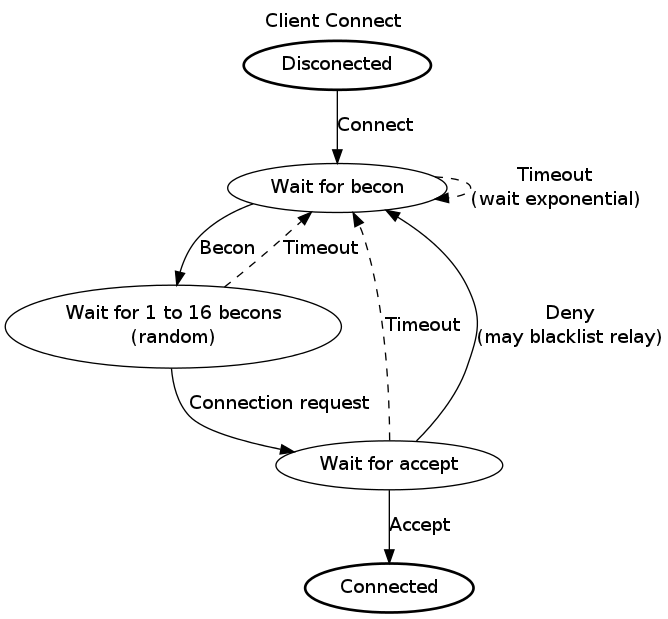
\includegraphics[width=0.4\textwidth, keepaspectratio=true]{images/Network_Connect.png}
  \end{center}
  \caption[Network Connection]{Network connection}
  \label{fig:net_connect}
  \vspace{-10pt}
\end{wrapfigure}

There are two main categories of address registration in networks. The first actively requests
addresses from a central source using the DL layer broadcast (\eg \ac{DHCP}). The second listens to the
network and tries to attempt to join using the information learned (\eg \ac{NDP}). It was decided to
use a mixed model for the Respire network in an attempt to optimise the network.

\begin{wrapfigure}{r}{0.3\textwidth}
  \vspace{-10pt}
  \begin{center}
    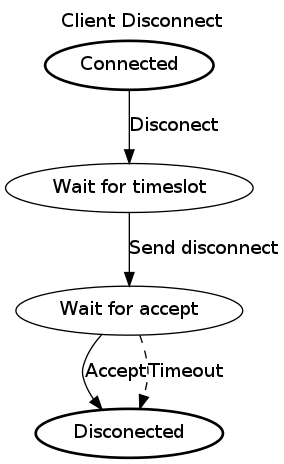
\includegraphics[width=0.2\textwidth, keepaspectratio=true]{images/Network_Disconnect.png}
  \end{center}
  \caption[Network Disconnect]{Network disconnect}
  \label{fig:net_disconect}
  \vspace{-10pt}
\end{wrapfigure}

% TODO Add info on the event if the address is taken on attempted use before first attempt
Periodic broadcasts are sent with next available address to be used by a new child device. An
unconnected node listens for a broadcast, by first-found or strongest-signal, and then randomly
waits 1 to 16 more broadcasts from that relay, this prevent self denial of service on a full network
reset. After the wait the node will then transmit a connection request in the \ac{TDMA} block defined by
the address in the broadcast field. The relay will reply with accept or deny, with the denial reason. In failure, due
to packet collision by another device trying to connect, the 1 to 16 delay is repeated. If the denial
reason suggests an inability to connect to that relay, it should be blacklisted. This design allows
nodes to know if a network is accepting connections, the address to use and the additional
information in the broadcast (all before connecting) and also minimises denial of service and packet
collisions. Again this design allows effective device sleeping as during the wait periods there is a
known duration of sleep (Figure \ref{fig:net_connect}).

\begin{wrapfigure}{r}{0.4\textwidth}
  \vspace{-10pt}
  \begin{center}
    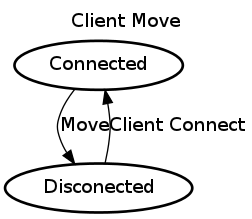
\includegraphics[width=0.3\textwidth, keepaspectratio=true]{images/Network_Move.png}
  \end{center}
  \caption[Network Move]{Network move}
  \vspace{-10pt}
\end{wrapfigure}

On the device wishing to disconnect from the network, a simple disconnect request is sent. If the
relay does not receive an accept, it should still disconnect and assume the relay will remove it
through a timeout (Figure \ref{fig:net_disconect}). This additional information sent to the parent allows fast reuse of the
time division slot in situations, such as busy hospital wards, where the parent is at capacity.
On the device wishing to transfer to a different relay in the same network, the device will first send a
disconnect request- with intent to transfer- to the current relay. Whether the last packet is received
or not, the device connects to the new relay. The last packet received from the previous relay
provides the ability, currently not used, for quick switching.

\subsubsection{Addressing}
Along with a globally unique \ac{DL} Address the network layer will register for a transient network
address. This address has several purposes: it enables packet routing, is used as the \ac{TDMA} time slot
and controls the bandwidth allocation.


The address is a single byte divided into a upper and lower nibble. The upper nibble identifies the
connected relay and the lower identifies the node within the relay. This small address range was
chosen as after a network surpasses 256 nodes and relays it also surpasses the available bandwidth
for that channel. Several separate networks on independent channels would allow more than 255
devices.


The \ac{TDMA} time slot is decided by the device address. The initial period is separated into 128 relay
blocks which in turn are separated into 128 node blocks. This system guarantees that every device
connected to the network, even across relays, has a unique time slot to transmit in. The nodes' radio
use is then condensed into a short period, allowing long periods of uninterrupted sleep, reducing
duty.


\subsubsection{\acf{DL} Layer Monitoring}
With more knowledge than the \ac{DL} layer, the network layer can make better decisions on power
management and buffer control than the \ac{DL} layer. It is also important for the network layer to be
aware of the \ac{DL} layer's state in the project as it is so intertwined in the \ac{PHY} layer and the thus power
management.

\subsubsection{Link Management}
The network layer also provides keep-alive and retransmission functions to prevent relays timing out
a device or to control retransmission of key messages.


\subsection{Application Layer}
The application layer is separated into three parts: real-time data, bulk data and administration data.
This separation is based around the differing network patterns that are needed.


\subsubsection{Real-time Data}

\begin{wrapfigure}{r}{0.6\textwidth}
  \vspace{-10pt}
  \begin{center}
    \begin{bytefield}{32}
      \bitheader[b]{0,7,8,15,16,23,24,31} \\
      \bitbox{6}{Time} & \bitbox{14}{Sample 1 X} & \bitbox{12}{Sample 1 Y} \\
      \bitbox{2}{} & \bitbox{14}{Sample 1 Z} & \bitbox{14}{Sample 2 X} & \bitbox{2}{} \\
      \wordbox[lrt]{1}{Samples 2, 3 and 4} \\
      \skippedwords \\
      \wordbox[lrb]{1}{} \\
      \bitbox{4}{} & \bitbox{14}{Sample 5 Y} & \bitbox{14}{Sample 5 Z} \\
    \end{bytefield}
  \end{center}
  \caption[Real-Time Packet]{Real-time packet}
  \label{rt_packet}
\end{wrapfigure}

Real-time data is buffered and transmitted with no retransmission or confirmation. This data has
consciously been produced so any attempt to retransmit may overflow the buffers.
As the requirement for this real-time data is 3x14bits at a minimum of 12.5Hz, I
have decided to optimise the packet design to meet the specific characteristics of
the \ac{NRF24} as it allows close alignment. With the \ac{NRF24}'s 3 packet pipeline
and maximum packet size of 32bytes combined with the design for independent packets
a value of 5 full samples a packet (less than 27bytes) was chosen (Figure \ref{rt_packet}). In addition,
a 7-bit time field is included to allowing the receiver to determine the exact time
the samples are valid, providing an accuracy of 63miliseconds within a 4 second period.


\subsubsection{Bulk Data}
Bulk data is sent via a request to the relay for a bulk \ac{TDMA} time slot. The data is then fragmented
and sent with confirmation received via the administration interface. A timeout and full
retransmission will be initially implemented but this does not prevent a more effective sliding
window algorithm implementation.

\subsubsection{Administration}
In every beacon there is a bitmap informing every node whether, during their \ac{TDMA} slot, they will
be requested to receive a packet or not. Data sent and received via the administration channel is
confirmed and on timeout, retransmitted. Data sent via this channel takes priority over the normal
real-time data flow through the \ac{TDMA} slot; it does not interfere with the bulk data \ac{TDMA} slot.


\section{Duty Cycle}
The power consumption of a device is determined by its power usage and how long the device is on
for. Thus reducing the power needed during use and/or reducing the period of use will help meet
the requirements of a low-power device. The percentage of time on as a ratio of the total time is
referred to as the duty cycle. In the Respire during use the radio is the main consumer of power,
therefore reducing its duty cycle will best enable lower power needs. The use of \ac{TDMA} in the project
assists in reducing the device's duty cycle as it allows the radio to know when it is not required to
operate, and therefore permits prolonged use of the low power states.


\section{Power Management}
With each chip in the Respire having its own set of sleep states and particular sequences moving
between them, it is imperative that there is a clear and correct state machine for controlling them.


The EFM32 microcontroller contains 4 sleep states as well as independent clocks and individually
enabled peripherals. This complexity brings great value with its low power but forces complex
configuration and undefined errors if incorrectly implemented. As several states (2, 3 and 4) in the
\ac{MCU} disable the \ac{SPI}'s clock, it is required that the \ac{SPI} is reconfigured and the clock started
manually again. The EFM32 however has a \ac{PRS} that enables peripherals on
the chip to interact with each other when the \ac{MCU} is off. This feature allows the radio
\ac{FIFO} transmit buffer to be loaded, the chip to sleep and then independently the
\ac{RTC} to enable the \ac{GPIO} line to transmit the packet at the precise
time without the need to wake the \ac{MCU}. There are however several aspects of the design
of the EFM32G series\cite{EFM32Ref} that mean extra reconfiguration is needed entering
and leaving sleep states; these have caused many problems and complexities during
development of the current project.


An important feature on the \ac{NRF24} radio is that it can maintain its state allowing \ac{FIFO} accesses
without the need for the receiver or transmitter to be active. This greatly reduces the power
consumption as both receiving and transmitting states require significant power.


\section{The \acf{OS}}

\begin{wrapfigure}{r}{0.6\textwidth}
  \vspace{-10pt}
  \begin{center}
    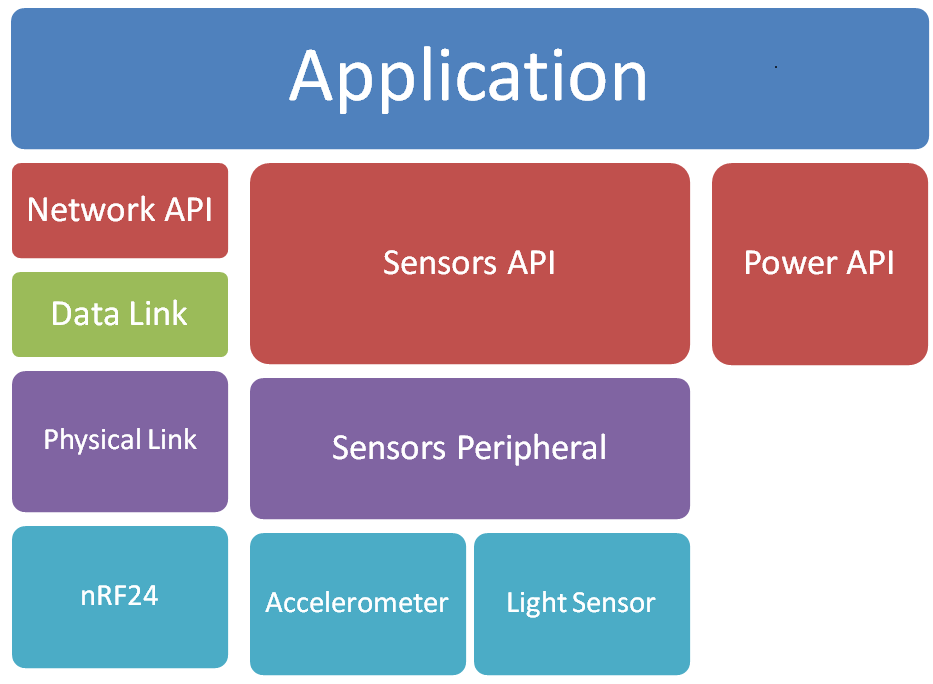
\includegraphics[width=0.5\textwidth, keepaspectratio=true]{images/archatechture.png}
  \end{center}
  \caption[System Architecture]{System Architecture}
  \vspace{-10pt}
\end{wrapfigure}

\subsection{Modularity}
Following the design of the modular system it was key to implement to system from the ground up
to support this reduced coupling. Each module is given and initialisation and de-initialisation call to
enable peripherals and data structures to be configured and also so after use all unnecessary
systems can be powered down. This de-initialisation was found to be most important during
development as the many of the peripherals continue to interact with the system after use, causing
faults.

Each module then has a public \ac{API} to simplify and abstract its internal processes. This is also
important as the C programming module does not support the protection of functions or variables
and so the use and separation of public interfaces allowed immediate warning throughout the use of
the compiler when functions or data where misused. The \ac{API} was used to abstract all data stored
locally in each module by the use of getters and setter forcing data localisation through the use of
coding conventions. These abstractions can be easily compiled out so does not incur a performance
reduction.

% TODO
\clearpage
\clearpage
\lstset{language=[ANSI]C, frame=single, caption={Module \ac{API}}}
\begin{lstlisting}
/* Called to (re)configure the module */
void init(void);
/* Called to configure the module only if not
 * already done so
 */
void required(void);
/* Called to asses the minimum sleep state the
 * system can achive */
sleep min_sleep(void);
/* Called to (re)configure the module if needed
 * after a sleep state */
void wakeup(sleep from);
/* Called to unconfigure the module */
void deinit(void);
\end{lstlisting}

The modularity of the code also assisted in reusability and supported the use of a
readable single code base. The use of a pre-processor was used to facilitate the
entire system being hosted in a single code base, without the separation of node
and base station. A pre-processor can lead to complex and often hidden errors when
used without modularity and so could be used safely with the design.
Listing \ref{lst:PreProsError} show clearly that the pre-processor also aids the
programmer by producing compile time errors, saving the time required to flash the devices.

\begin{minipage}[b]{0.5\linewidth}
  \vspace{+10pt}
  \begin{center}
    \lstset{language=[ANSI]C, frame=single, caption={Run-time Configuration}}
    \begin{lstlisting}
if (function == BASE) {
  run_base();
} else if (function == NODE){
  run_node();
} else {
  exit(EXIT_FAILURE);
}
    \end{lstlisting}
    %\caption[ToDo]{ToDo}
  \end{center}
\end{minipage}
\hspace{0.1cm}
\begin{minipage}[b]{0.5\linewidth}
  \vspace{+10pt}
  \begin{center}
    \lstset{language=[ANSI]C, frame=single, caption={Compile-time Configuration}, label=lst:PreProsError}
    \begin{lstlisting}
#if FUNCTION == BASE
  run_base();
#elif function == NODE
  run_node();
#else
#error "Invalid 'FUNCTION'"
#endif
    \end{lstlisting}
    %\caption[ToDo]{ToDo}
  \end{center}
\end{minipage}

